\documentclass{standalone}
\usepackage{tikz}
\usepackage{xcolor}
\usetikzlibrary{patterns, positioning}
\usetikzlibrary{shapes.misc}
\usepackage[outline]{contour}
\contourlength{1.5pt} 


\begin{document}
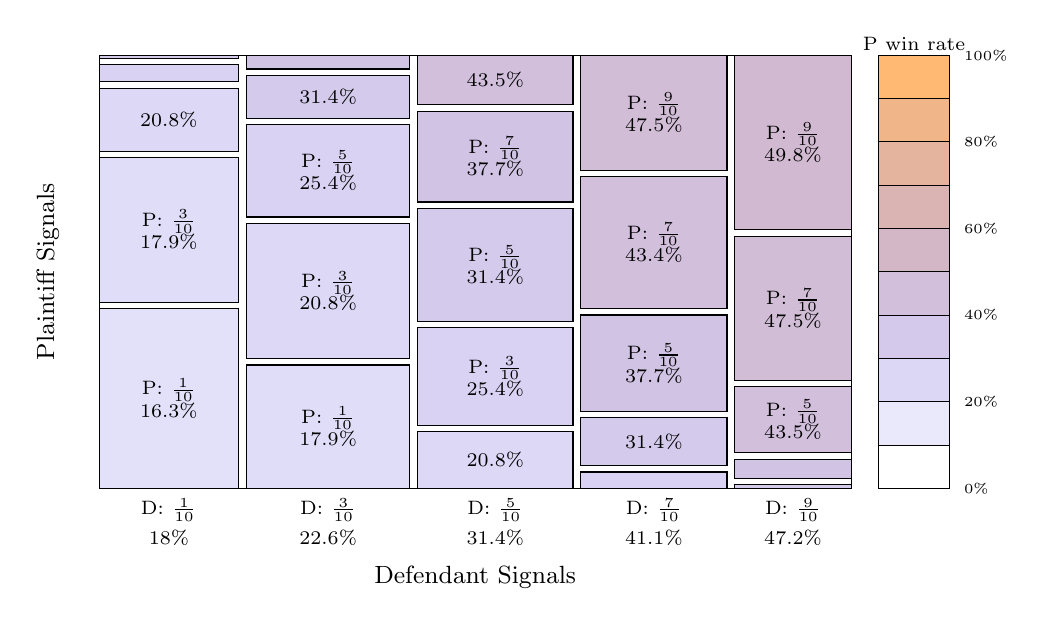
\begin{tikzpicture}
\newcommand{\DFractionOffset}{0.4}
\newcommand{\AxisLabelYAdjust}{-0.235}
\draw[draw=black] (0.6,2) rectangle (10.15,7.5);
\draw[fill=blue!84!orange!16!white!83!white, draw=black] (0.6,2) rectangle (2.3711,4.2859);
\draw (1.4855636045925307, 3.142957492536121) node[font=\scriptsize, text=black, align=center] {P: $\frac{1}{10}$\\ 16.3\%};
\draw[fill=blue!82!orange!18!white!82!white, draw=black] (0.6,4.3659) rectangle (2.3711,6.2013);
\draw (1.4855636045925307, 5.283615088902921) node[font=\scriptsize, text=black, align=center] {P: $\frac{3}{10}$\\ 17.9\%};
\draw[fill=blue!79!orange!21!white!81!white, draw=black] (0.6,6.2813) rectangle (2.3711,7.0826);
\draw (1.4855636045925307, 6.68194691509494) node[font=\scriptsize, text=black, align=center] {20.8\%};
\draw[fill=blue!75!orange!25!white!80!white, draw=black] (0.6,7.1626) rectangle (2.3711,7.3802);
\draw[fill=blue!69!orange!31!white!78!white, draw=black] (0.6,7.4602) rectangle (2.3711,7.5);
\draw (1.4855636045925307, 1.6) node[anchor=north, font=\scriptsize, text=black] {18\%};
\draw (1.4855636045925307, {1.6 + \DFractionOffset}) node[anchor=north, font=\scriptsize, text=black] {D: $\frac{1}{10}$};
\draw[fill=blue!82!orange!18!white!82!white, draw=black] (2.4711,2) rectangle (4.5461,3.5667);
\draw (3.5085968409119292, 2.7833306990687783) node[font=\scriptsize, text=black, align=center] {P: $\frac{1}{10}$\\ 17.9\%};
\draw[fill=blue!79!orange!21!white!81!white, draw=black] (2.4711,3.6467) rectangle (4.5461,5.3663);
\draw (3.5085968409119292, 4.506488757621192) node[font=\scriptsize, text=black, align=center] {P: $\frac{3}{10}$\\ 20.8\%};
\draw[fill=blue!75!orange!25!white!80!white, draw=black] (2.4711,5.4463) rectangle (4.5461,6.623);
\draw (3.5085968409119292, 6.0346636109332055) node[font=\scriptsize, text=black, align=center] {P: $\frac{5}{10}$\\ 25.4\%};
\draw[fill=blue!69!orange!31!white!78!white, draw=black] (2.4711,6.703) rectangle (4.5461,7.2469);
\draw (3.5085968409119292, 6.974975103444873) node[font=\scriptsize, text=black, align=center] {31.4\%};
\draw[fill=blue!62!orange!38!white!76!white, draw=black] (2.4711,7.3269) rectangle (4.5461,7.5);
\draw (3.5085968409119292, 1.6) node[anchor=north, font=\scriptsize, text=black] {22.6\%};
\draw (3.5085968409119292, {1.6 + \DFractionOffset}) node[anchor=north, font=\scriptsize, text=black] {D: $\frac{3}{10}$};
\draw[fill=blue!79!orange!21!white!81!white, draw=black] (4.6461,2) rectangle (6.6178,2.7197);
\draw (5.6319510182991355, 2.359864523417183) node[font=\scriptsize, text=black, align=center] {20.8\%};
\draw[fill=blue!75!orange!25!white!80!white, draw=black] (4.6461,2.7997) rectangle (6.6178,4.038);
\draw (5.6319510182991355, 3.418861033877247) node[font=\scriptsize, text=black, align=center] {P: $\frac{3}{10}$\\ 25.4\%};
\draw[fill=blue!69!orange!31!white!78!white, draw=black] (4.6461,4.118) rectangle (6.6178,5.5575);
\draw (5.6319510182991355, 4.837756160929247) node[font=\scriptsize, text=black, align=center] {P: $\frac{5}{10}$\\ 31.4\%};
\draw[fill=blue!62!orange!38!white!76!white, draw=black] (4.6461,5.6375) rectangle (6.6178,6.7912);
\draw (5.6319510182991355, 6.214342713457378) node[font=\scriptsize, text=black, align=center] {P: $\frac{7}{10}$\\ 37.7\%};
\draw[fill=blue!57!orange!43!white!74!white, draw=black] (4.6461,6.8712) rectangle (6.6178,7.5);
\draw (5.6319510182991355, 7.185583062988194) node[font=\scriptsize, text=black, align=center] {43.5\%};
\draw (5.6319510182991355, 1.6) node[anchor=north, font=\scriptsize, text=black] {31.4\%};
\draw (5.6319510182991355, {1.6 + \DFractionOffset}) node[anchor=north, font=\scriptsize, text=black] {D: $\frac{5}{10}$};
\draw[fill=blue!75!orange!25!white!80!white, draw=black] (6.7178,2) rectangle (8.5736,2.2077);
\draw[fill=blue!69!orange!31!white!78!white, draw=black] (6.7178,2.2877) rectangle (8.5736,2.8959);
\draw (7.645701086597638, 2.591776398940399) node[font=\scriptsize, text=black, align=center] {31.4\%};
\draw[fill=blue!62!orange!38!white!76!white, draw=black] (6.7178,2.9759) rectangle (8.5736,4.2016);
\draw (7.645701086597638, 3.5887580700723536) node[font=\scriptsize, text=black, align=center] {P: $\frac{5}{10}$\\ 37.7\%};
\draw[fill=blue!57!orange!43!white!74!white, draw=black] (6.7178,4.2816) rectangle (8.5736,5.9616);
\draw (7.645701086597638, 5.12163012667745) node[font=\scriptsize, text=black, align=center] {P: $\frac{7}{10}$\\ 43.4\%};
\draw[fill=blue!53!orange!47!white!72!white, draw=black] (6.7178,6.0416) rectangle (8.5736,7.5);
\draw (7.645701086597638, 6.770805128243128) node[font=\scriptsize, text=black, align=center] {P: $\frac{9}{10}$\\ 47.5\%};
\draw (7.645701086597638, 1.6) node[anchor=north, font=\scriptsize, text=black] {41.1\%};
\draw (7.645701086597638, {1.6 + \DFractionOffset}) node[anchor=north, font=\scriptsize, text=black] {D: $\frac{7}{10}$};
\draw[fill=blue!69!orange!31!white!78!white, draw=black] (8.6736,2) rectangle (10.15,2.0478);
\draw[fill=blue!62!orange!38!white!76!white, draw=black] (8.6736,2.1278) rectangle (10.15,2.371);
\draw[fill=blue!57!orange!43!white!74!white, draw=black] (8.6736,2.451) rectangle (10.15,3.2908);
\draw (9.4117833046179, 2.8708778922930382) node[font=\scriptsize, text=black, align=center] {P: $\frac{5}{10}$\\ 43.5\%};
\draw[fill=blue!53!orange!47!white!72!white, draw=black] (8.6736,3.3708) rectangle (10.15,5.2038);
\draw (9.4117833046179, 4.287306052280548) node[font=\scriptsize, text=black, align=center] {P: $\frac{7}{10}$\\ 47.5\%};
\draw[fill=blue!50!orange!50!white!72!white, draw=black] (8.6736,5.2838) rectangle (10.15,7.5);
\draw (9.4117833046179, 6.391916016546875) node[font=\scriptsize, text=black, align=center] {P: $\frac{9}{10}$\\ 49.8\%};
\draw (9.4117833046179, 1.6) node[anchor=north, font=\scriptsize, text=black] {47.2\%};
\draw (9.4117833046179, {1.6 + \DFractionOffset}) node[anchor=north, font=\scriptsize, text=black] {D: $\frac{9}{10}$};
\node[font=\small, text=black] at (5.375, {1.1 + \AxisLabelYAdjust}) {Defendant Signals};
\node[font=\small, text=black, rotate=90] at (-0.050000000000000044, 4.75) {Plaintiff Signals};
\draw[draw=black] (10.5,2) rectangle (11.4,7.5);
\draw (10.95, 7.65) node[font=\scriptsize, text=black] {P win rate};
\draw[fill=blue!100!orange!0!white!88!white, draw=black] (10.5,2) rectangle (11.4,2.55);
\draw[fill=blue!89!orange!11!white!84!white, draw=black] (10.5,2.55) rectangle (11.4,3.1);
\draw[fill=blue!78!orange!22!white!81!white, draw=black] (10.5,3.1) rectangle (11.4,3.65);
\draw[fill=blue!67!orange!33!white!77!white, draw=black] (10.5,3.65) rectangle (11.4,4.2);
\draw[fill=blue!56!orange!44!white!73!white, draw=black] (10.5,4.2) rectangle (11.4,4.75);
\draw[fill=blue!44!orange!56!white!70!white, draw=black] (10.5,4.75) rectangle (11.4,5.3);
\draw[fill=blue!33!orange!67!white!66!white, draw=black] (10.5,5.3) rectangle (11.4,5.85);
\draw[fill=blue!22!orange!78!white!62!white, draw=black] (10.5,5.85) rectangle (11.4,6.4);
\draw[fill=blue!11!orange!89!white!59!white, draw=black] (10.5,6.4) rectangle (11.4,6.95);
\draw[fill=blue!0!orange!100!white!55!white, draw=black] (10.5,6.95) rectangle (11.4,7.5);
\draw (11.46, 2) node[anchor=west, font=\tiny, text=black] {0\%};
\draw (11.46, 3.1) node[anchor=west, font=\tiny, text=black] {20\%};
\draw (11.46, 4.2) node[anchor=west, font=\tiny, text=black] {40\%};
\draw (11.46, 5.3) node[anchor=west, font=\tiny, text=black] {60\%};
\draw (11.46, 6.4) node[anchor=west, font=\tiny, text=black] {80\%};
\draw (11.46, 7.5) node[anchor=west, font=\tiny, text=black] {100\%};


\end{tikzpicture}
\end{document}